%======================================================================
%  Improving extension services through non-monetary incentives
%  Manuscript skeleton. Body text is written by hand; everything inside
%  the float environments is generated by the Stata pipeline in do/ and
%  lands in tmp/. Floats and their order follow JICA-Ghana-研究会.tex.
%======================================================================
\documentclass[11pt]{article}

\usepackage[margin=1in]{geometry}
\usepackage{graphicx}
\usepackage{booktabs}
\usepackage{array}
\usepackage{amsmath}
\usepackage{caption}
\usepackage{float}
\usepackage{pdflscape}
\usepackage{setspace}
\doublespacing
\usepackage[style=apa, backend=biber, natbib=true]{biblatex}
\DeclareLanguageMapping{english}{english-apa}
\addbibresource{references.bib}
\graphicspath{{tmp/}}

% every generated fragment is a bare tabular; this scales the wide ones
\newcommand{\fittable}[1]{\resizebox{\textwidth}{!}{\input{#1}}}
\captionsetup[table]{skip=4pt}
\captionsetup{font=small,labelfont=bf}
\newcommand{\tnote}[1]{\par\vspace{2pt}{\footnotesize\textit{Note:} #1}}

\title{Improving extension services through non-monetary incentives: Experimental evidence from Ghana}
\author{Kazushi Takahashi \and Wataru Kodama \and Yukichi Mano}
\date{\today}

\begin{document}

\maketitle

\begin{abstract}
We study the impacts of non-monetary incentives on agricultural extension agents (AEA) in Ghana. 
\end{abstract}

\clearpage

\section{Introduction}
Improving agricultural productivity requires the adoption of new technologies, such as improved seeds, chemical fertilizers, and appropriate crop management practices \citep{takahashi_technology_2020}. Since technology development, adoption, and diffusion involve externality, public institutions play a central role. Public agricultural extension workers are key actors in disseminating technologies...

%======================================================================
\section{Experimental design and data}\label{sec:design}
%======================================================================

\begin{figure}[H]
\centering
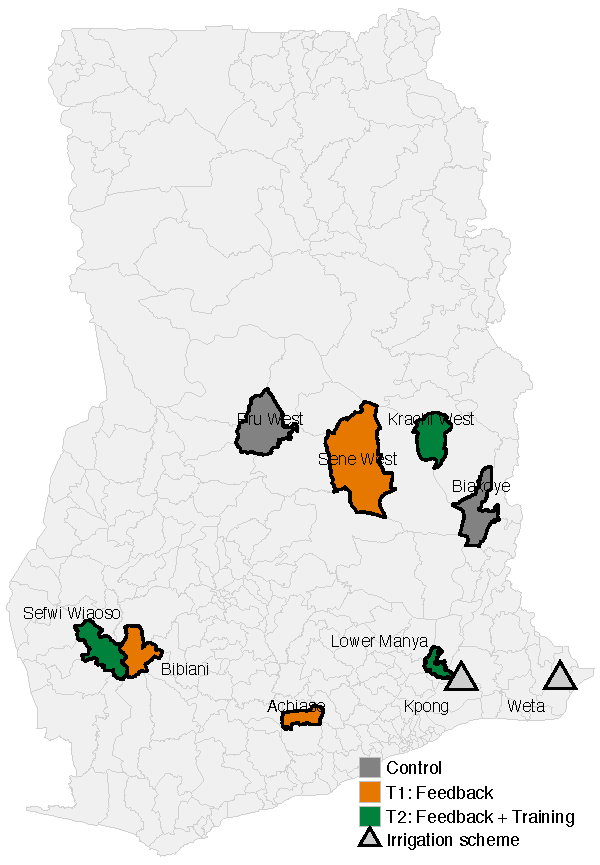
\includegraphics[width=0.55\textwidth]{fig_map_study_areas.pdf}
\caption{Study areas}
\label{fig:map}
\end{figure}

\begin{table}[H]
\centering
\caption{Sample size by district}
\label{tab:obs}
\resizebox{\textwidth}{!}{%
\begin{tabular}{llccccccc}
\hline
Province & District & \multicolumn{2}{c}{Baseline} & \multicolumn{2}{c}{Endline} & \multicolumn{2}{c}{Analysis} & Treatment\\
 & & Farmers & AEAs & Farmers & AEAs & Farmers & AEAs & \\ \hline
Bono East Region & Pru West &   40 &   4 &   39 &   4 &   39 &   4 & C \\
Bono East Region & Sene West &   40 &   4 &   39 &   4 &   39 &   4 & T1 \\
Eastern Region & Achiase &   33 &   4 &   34 &   4 &   33 &   4 & T1 \\
Eastern Region & Kpong Irrigation &    2 &   1 &    2 &   1 &    0 &   0 & C \\
Eastern Region & Lower Manya &   17 &   2 &   18 &   2 &   17 &   2 & T2 \\
Oti Region & Biakoye &   52 &   7 &   51 &   6 &   50 &   6 & C \\
Oti Region & Krachi West &   59 &   7 &   63 &   7 &   59 &   7 & T2 \\
Volta Region & Ketu North &   10 &   1 &   10 &   1 &    0 &   0 & C \\
Western North region & Bibiani &   79 &   8 &   79 &   8 &   79 &   8 & T1 \\
Western North region & Sefwi Wiaoso &   58 &   6 &   59 &   6 &   57 &   6 & T2 \\
\hline  & & 390 & 44 & 394 & 43 &  373 &  41 & \\ \hline

\end{tabular}}
\end{table}

\begin{table}[H]
\centering
\caption{AEA characteristics}
\label{tab:aeachar}
\fittable{tmp/desc_arm_aea_char}
\end{table}

\begin{table}[H]
\centering
\caption{AEA motivation and performance}
\label{tab:aeaall}
\fittable{tmp/desc_arm_aea_all}
\end{table}

\begin{table}[H]
\centering
\caption{Farm households and inputs}
\label{tab:farmchar}
\fittable{tmp/desc_arm_farmer_noirr}
\end{table}

\begin{table}[H]
\centering
\caption{Rice production and technology}
\label{tab:farmprod}
\fittable{tmp/desc_arm_farmer_noirr_b}
\end{table}

\begin{table}[H]
\centering
\caption{Farmer--AEA contact}
\label{tab:contact}
\fittable{tmp/desc_arm_contact}
\end{table}

\clearpage
%======================================================================
\section{Measuring AEA performance}\label{sec:performance}
%======================================================================

\begin{figure}[H]
\centering
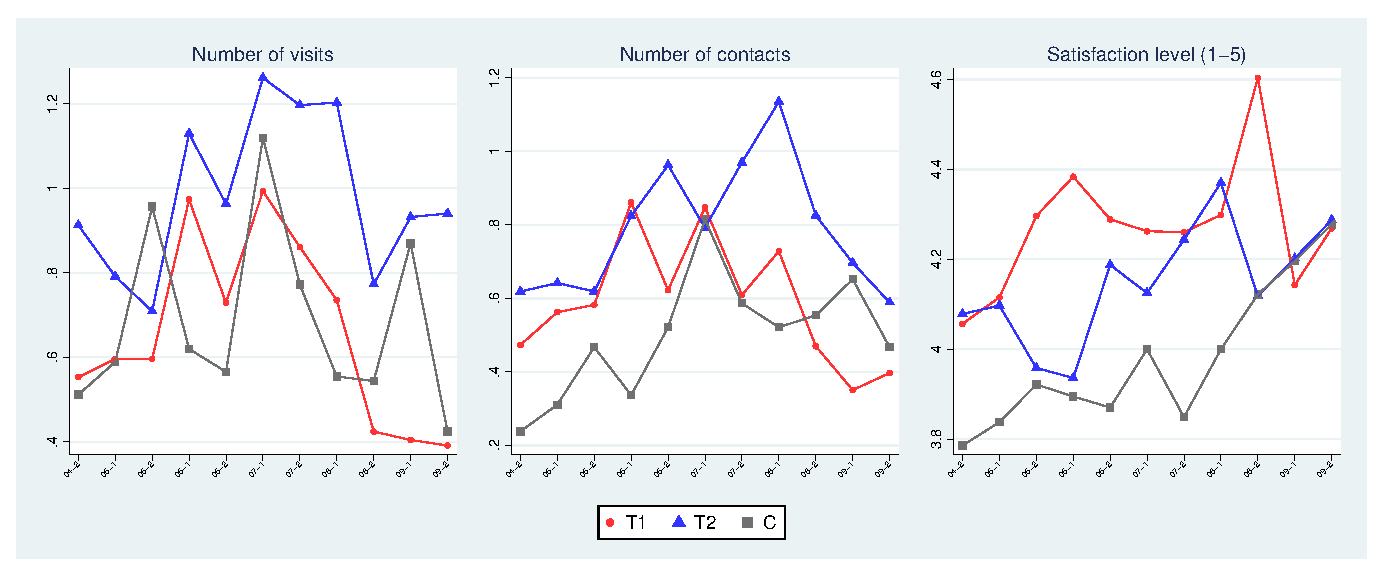
\includegraphics[width=0.85\textwidth]{b_basic.eps}
\caption{Extension activity over the season}
\label{fig:bwbasic}
\end{figure}

\begin{figure}[H]
\centering
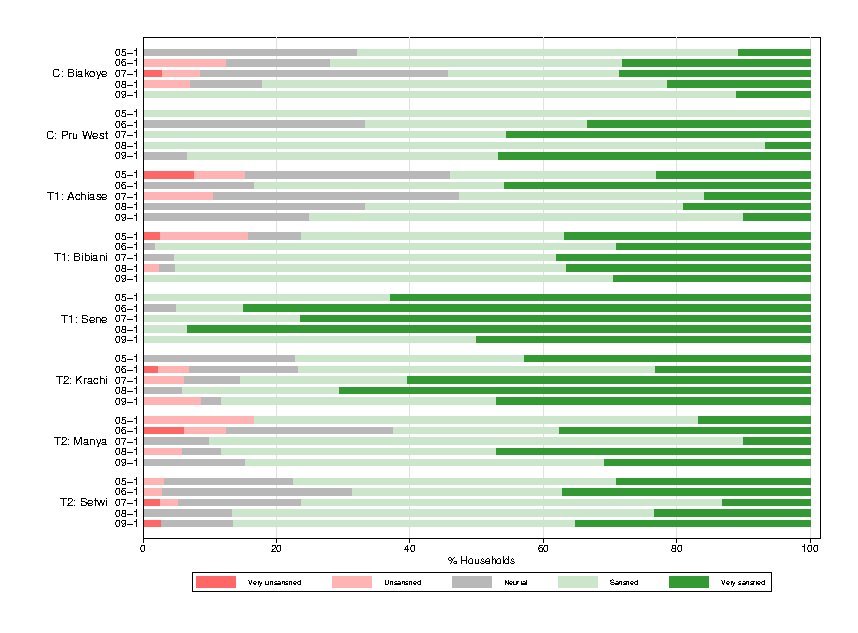
\includegraphics[width=0.85\textwidth]{b_satisfy.eps}
\caption{Satisfaction with extension service, by district and round}
\label{fig:bwsatisfy}
\end{figure}

\begin{figure}[H]
\centering
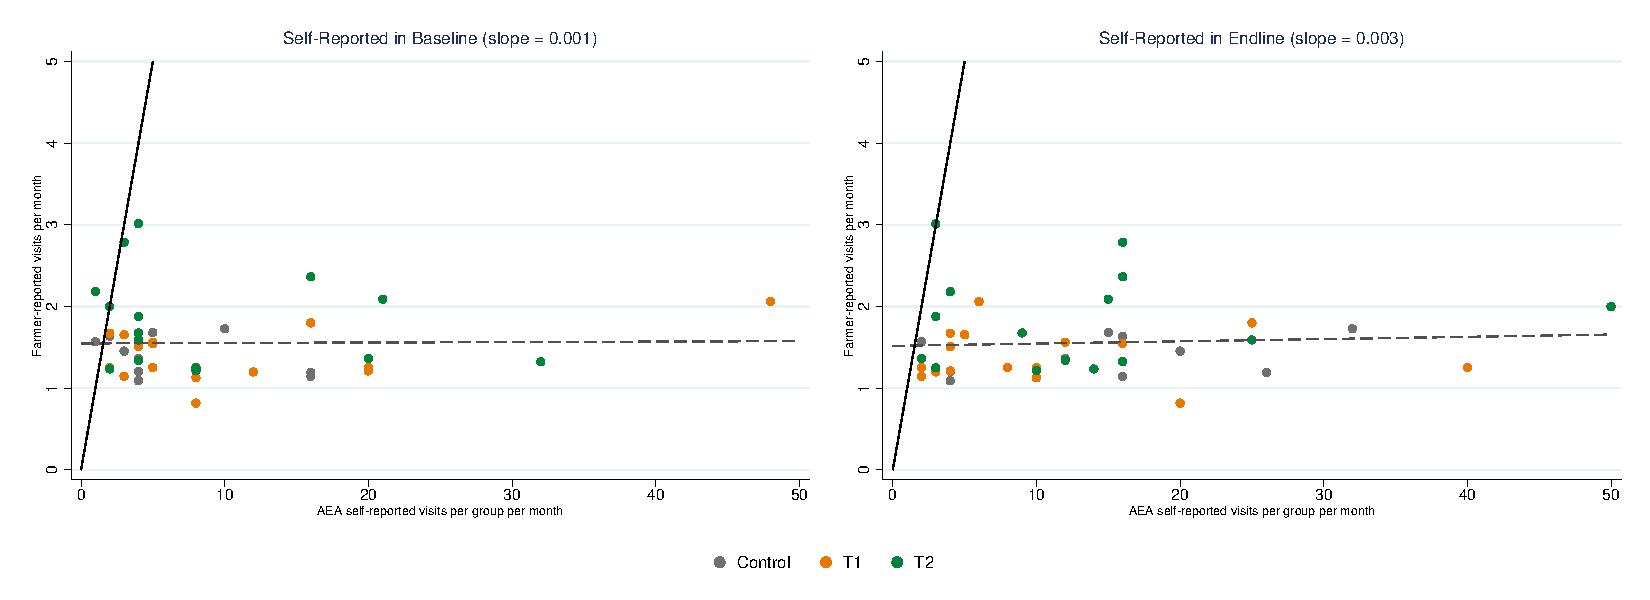
\includegraphics[width=0.85\textwidth]{fig_selfrep_farmer.pdf}
\caption{AEA effort: self-reported versus farmer-reported visits}
\label{fig:selfrep}
\end{figure}

\begin{figure}[H]
\centering
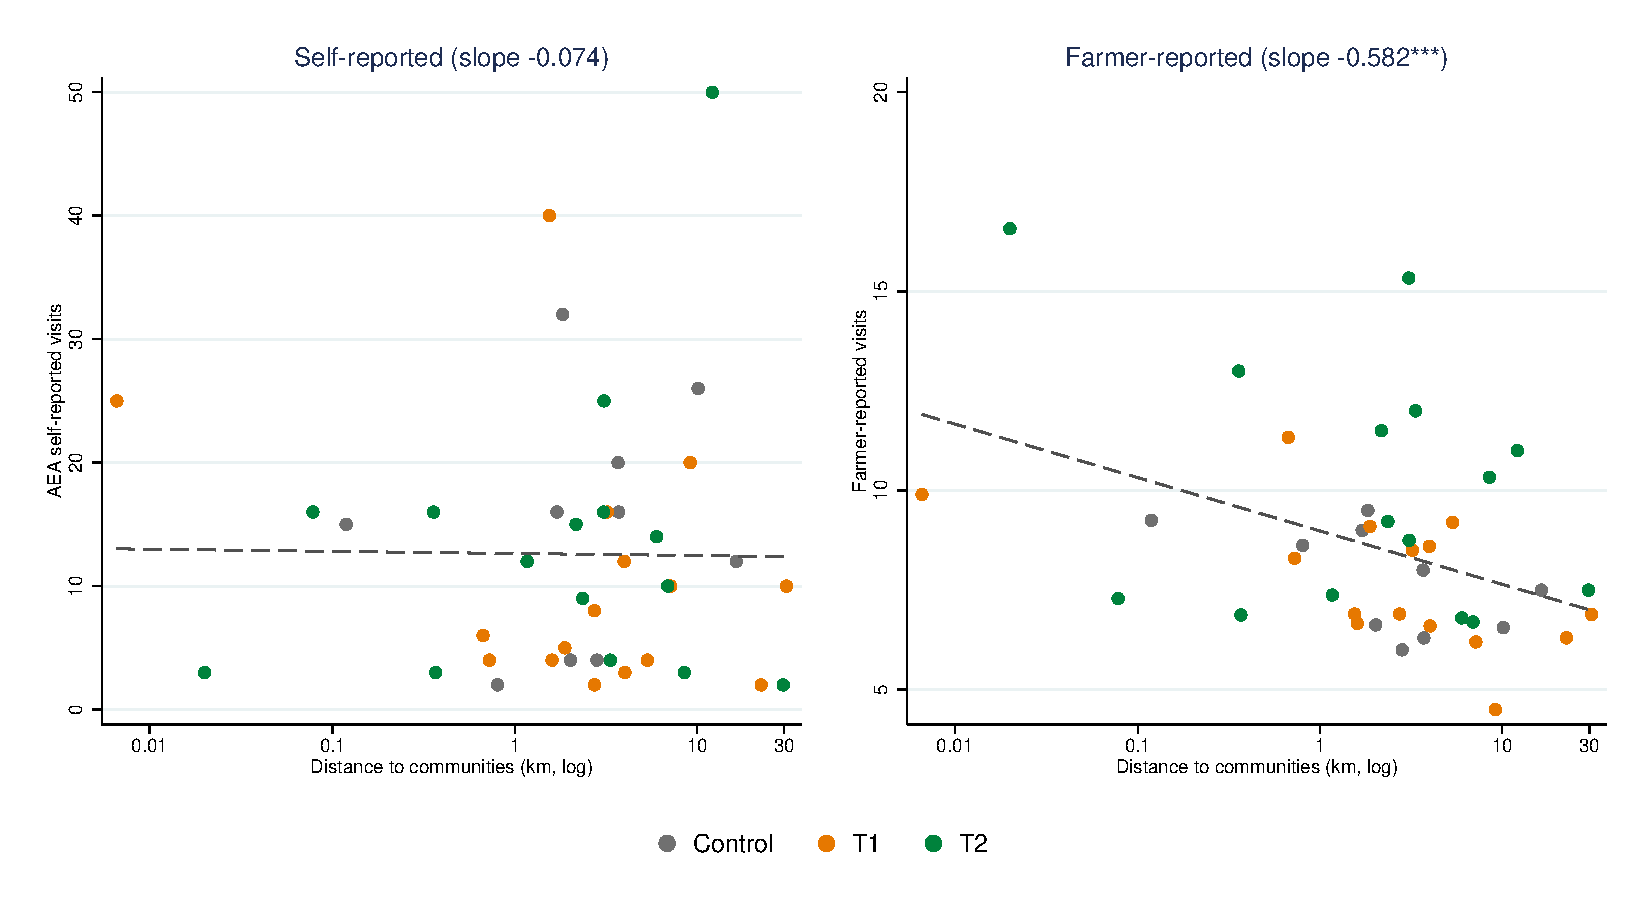
\includegraphics[width=0.85\textwidth]{fig_dist_visits.pdf}
\caption{AEA effort: distance to the communities served}
\label{fig:distvisits}
\end{figure}

\begin{table}[H]
\centering
\caption{Effort reported by farmers, bi-weekly rounds}
\label{tab:bweffort}
\fittable{tmp/bw_effort_v2}
\end{table}

\begin{table}[H]
\centering
\caption{Satisfaction with extension service, bi-weekly rounds}
\label{tab:bwsatisfy}
\fittable{tmp/bw_satisfy_v2}
\end{table}

\begin{table}[H]
\centering
\caption{Content of the extension service, bi-weekly rounds}
\label{tab:bwcontent}
\fittable{tmp/bw_content_a}
\end{table}

\begin{figure}[H]
\centering
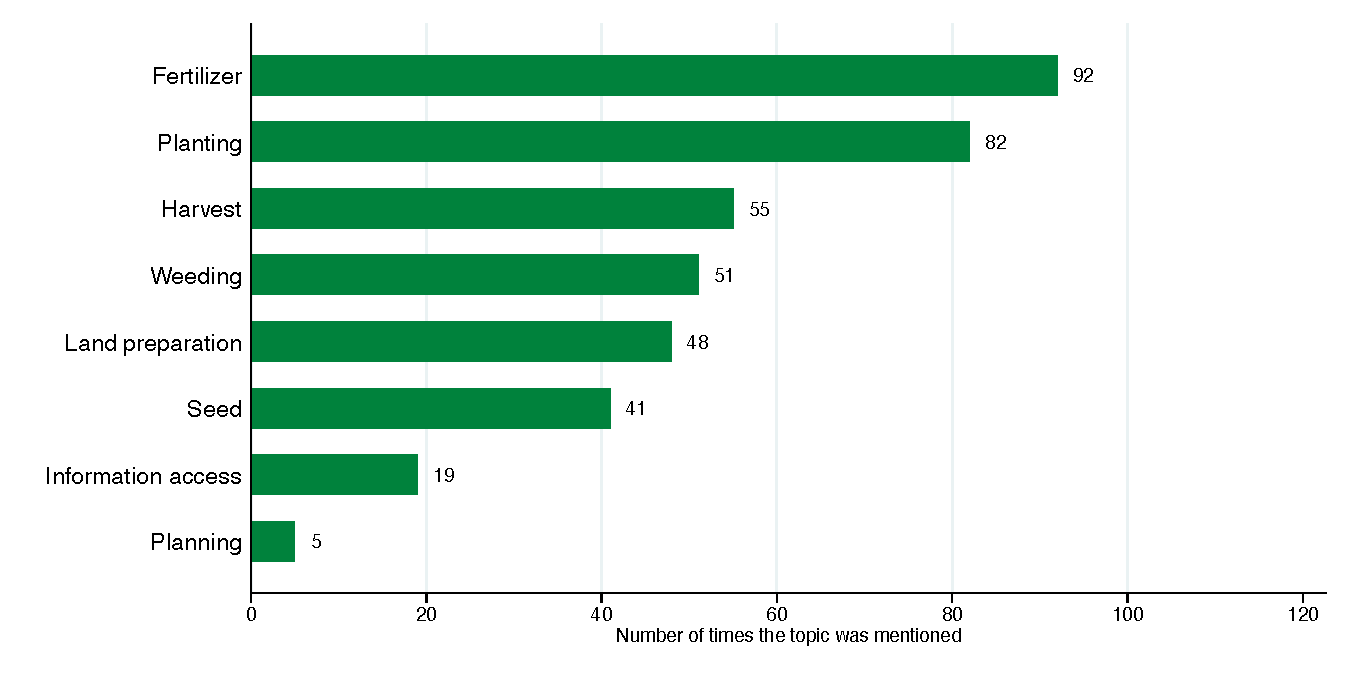
\includegraphics[width=0.85\textwidth]{fig_advice_themes.pdf}
\caption{What the advice was about}
\label{fig:advice}
\end{figure}

\clearpage
%======================================================================
\section{AEA and farm level impacts}\label{sec:impacts}
%======================================================================

\begin{table}[H]
\centering
\caption{AEA motivation and locus of control}
\label{tab:aeaattitude}
\fittable{tmp/e_aea_attitude}
\end{table}

\begin{table}[H]
\centering
\caption{AEA knowledge, effort and job satisfaction}
\label{tab:aeaeffort}
\fittable{tmp/e_aea_effort}
\end{table}

\begin{table}[H]
\centering
\caption{Farm production and income}
\label{tab:prod}
\fittable{tmp/e_farmer_prod}
\end{table}

\begin{table}[H]
\centering
\caption{Farm production and income, controlling for technology}
\label{tab:prodtech}
\fittable{tmp/e_farmer_prod_tech}
\end{table}

\begin{table}[H]
\centering
\caption{Input use}
\label{tab:inputs}
\fittable{tmp/e_farmer_inputs}
\end{table}

\begin{table}[H]
\centering
\caption{Adoption of management practices}
\label{tab:practice}
\fittable{tmp/e_farmer_practice}
\end{table}

\begin{table}[H]
\centering
\caption{Labour use, by who does the work}
\label{tab:laboursex}
\fittable{tmp/e_labour_sex}
\end{table}

\begin{table}[H]
\centering
\caption{Labour use, by operation}
\label{tab:labourops}
\fittable{tmp/e_labour_ops}
\end{table}

\clearpage
%======================================================================
\section{Conclusion}\label{sec:conclusion}
%======================================================================

\clearpage
\printbibliography

\end{document}
